% ---------------------------------------------------
%
% Trabajo de Fin de Grado. 
% Author: Alejandro Hernández Padrón. 
% Capítulo: Tecnologías utilizadas en el Trabajo de Fin de Grado. 
% Fichero: Cap2_Technology.tex
%
% ----------------------------------------------------
%

\cleardoublepage
\chapter{Herramientas y Tecnologías} \label{chap:Tecnologias} 

Este capítulo tiene como objetivo presentar las distintas herramientas software y tecnologías empleadas por el alumno en el desarrollo de \ULLNavigation{}.

\section{Introduccion}

A continuación se explicarán brevemente las distintas herramientas software utilizadas en el proyecto. 

\subsection{Android Studio}

Android Studio \cite{URL::AndroidStudio} es el IDE (Entorno de Desarrollo Integrado) oficial para el desarrollo de aplicaciones en Android, basado en IntelliJ IDEA \cite{URL::IntelliJIDEA}. Android Studio ofrece una serie de funcionalidades que han facilitado a la desarrolladora numerosas tareas, entre las cuales podemos destacar:


\begin{itemize}
\item Un sistema de compilación basado en Gradle\cite{URL::Gradle} que ha simplificado tanto la inserción de dependencias de las distintas librerías que se han tenido que utilizar, como la compilación de la aplicación.
\item Un emulador rápido y fácil de utilizar que ha ayudado a visualizar las distintas pantallas durante el desarrollo aunque no ha sido de mucha utilidad para probar el funcionamiento al ser dependiente la app de la tecnología Bluetooth.
\item La facilidad para publicar cambios a aplicaciones ya funcionando sin tener que eliminar y volver a crear un nuevo APK parando la app.
\item Un sistema de visualización de las diferentes pantallas muy completo, con soporte visual para añadir componentes y cambiar atributos fácilmente.
\item Un sistema de depuración, con una interfaz sencilla e intuitiva.
\end{itemize} 

\begin{figure}[h]
	\centering
	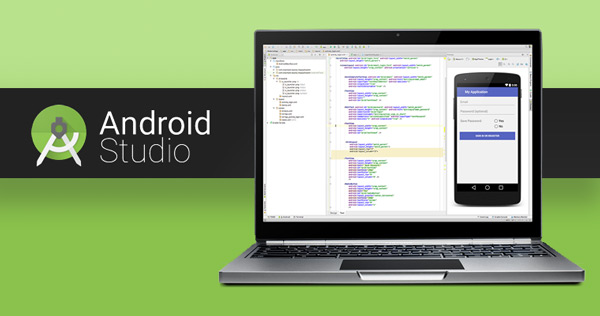
\includegraphics[width=0.6\linewidth]{androidstudio}
	\caption{Android Studio, un IDE flexible e intuitivo.}
	\label{fig:androidstudio}
\end{figure}

Se ha utilizado este IDE frente a otros como Eclipse + ADT \cite{URL::eclipseADT} debido a que en la actualidad es el IDE oficial con soporte de Google. Se ha preferido aprender a utilizar este entorno con vistas al futuro, ya que parece que se consolidará como el preferido para los desarrolladores Android.

\subsection{LaTex}

LaTeX es un sistema de composición de textos, orientado a la creación de documentos que presenten una alta calidad tipográfica. Por sus características y posibilidades, es usado especialmente en la generación de artículos y publicaciones científicas que incluyen, entre otros elementos, expresiones matemáticas, gráficos o figuras.


LaTeX está formado por un gran conjunto de macros de TeX, escrito por Leslie Lamport en 1984, con la intención de facilitar el uso del lenguaje de composición tipográfica, creado por Donald Knuth. LaTeX es software libre bajo licencia LPPL.


Se ha decidido utilizar este sistema debido al carácter profesional que aporta a los documentos. Ha sido una buena oportunidad para aprender a usar un sistema de composición de texto como este, ya que en un futuro puede ser beneficioso el saber manejar esta herramienta. 

Si bien es cierto, que el uso de esta herramienta frente a otros editores más familiares ha sido algo tedioso en el inicio, es verdad que una vez acostumbrada a su uso ha resultado ser muy eficaz. En el proceso de aprendizaje se recurrió principalmente a manuales por internet, alguno a destacar en español sería \cite{URL::manualLatex}

\subsection{Github}

GitHub\cite{URL::Github} es una forja (plataforma de desarrollo colaborativo) para alojar proyectos que utiliza el sistema de control de versiones Git. Utiliza el framework Ruby on Rails por GitHub, Inc. (anteriormente conocida como Logical Awesome). Desde enero de 2010, GitHub opera bajo el nombre de GitHub, Inc. El código se almacena de forma pública, aunque también se puede hacer de forma privada, creando una cuenta de pago.


Se ha decidido crear un repositorio en esta plataforma para poder llevar un control y una trazabilidad del proyecto. El tutor y el alumno han trabajado en este repositorio de manera conjunta. En el caso del tutor, principalmente para revisar el seguimiento semanal y llevar un control de las tareas. En el caso del alumno, para tener un repositorio donde subir los distintos elementos que se han ido generando a lo largo del trabajo. Aparte de este repositorio, también se ha abierto un segundo repositorio \cite{URL::repositorioAplicacion} asociado a la oficina del software libre (OSL) para subir el código una vez terminado como parte del programa de apoyo a trabajos finales libres (PATFL) \cite{URL::PATFL} de la ULL.


Mediante el uso de este repositorio, el alumno ha conseguido ampliar sus conocimientos en Git y familiarizarse con la interfaz de GitHub. Previamente se había utilizado como repositorios GitLab, SVN y RTC en otros proyectos, por lo que no ha sido una complicación mayor utilizar este sistema.

\section{Tecnologías utilizadas}

A continuación se revisan las distintas tecnologías utilizadas en el desarrollo de la aplicación.

\subsection{El Sistema Operativo Android}

Android es un sistema operativo que emplea Linux en la interfaz del hardware.  Los componentes del SO subyacentes se codifican en C o C++ pero las aplicaciones se desarrollan en Java. De esta manera Android asegura una amplia operatividad en una gran variedad de dispositivos debido a dos hechos: la interfaz en Linux ofrece gran potencia y funcionalidad para aprovechar el hardware, mientras que el desarrollo de las aplicaciones en Java permite que Android sea accesible para un gran número de programadores conocedores del código.

Este SO fue diseñado principalmente para dispositivos móviles con pantalla táctil: smartphones, tablets y otros dispositivos como televisores o automóviles. Fue desarrollado inicialmente por Android Inc., empresa que fue respaldada económicamente por Google y más tarde adquirida por esta misma empresa.

Actualmente tiene una gran comunidad de desarrolladores creando aplicaciones para extender la funcionalidad de los dispositivos. A fecha de hoy existen más de un millón de aplicaciones disponibles para la tienda oficial de Apps de Android, Google Play \cite{URL::GooglePlay} sin tener en cuenta las aplicaciones de otras tiendas no oficiales, como por ejemplo, la tienda de aplicaciones de Samsung Apps \cite{URL::SamsungApps}. XXX

\subsection{Realidad Aumentada}

La Realidad Aumentada(RA) o Augmented Reality(AR) en inglés es el término que se usa para definir la visión de un entorno físico del mundo real, a través de un dispositivo tecnológico. Este dispositivo, nos permite expandir nuestro mundo físico añadiendo capas de información digital generadas por un computador, como pueden ser imágenes, sonidos y videos a nuestra visión del entorno en tiempo real. RR

AR esta cambiando la manera en la que sus usuarios pueden ver el mundo, actualmente es una tecnología que se encuentra en auge debido a su enorme potencial, del cual podremos ver sus frutos en un futuro no muy lejano. RR

Sus posibles aplicaciones no tienen limites, pueden llegar desde reconocer plantas e incluso monumentos y mostrar información sobre lo que se esta viendo, hasta añadir información en tiempo real en una operación a un paciente, comprobar como queda un mueble en tu salón o sus aplicaciones para realizar videojuegos como podemos ver con el reciente éxito de Pokemon Go!. AA

A continuación se explicará en detalle:
\begin{itemize}
\item ¿Como funciona esta tecnología?
\item Diferencias entre Realidad Aumentada y Realidad Virtual
\item Realidad Mixta
\item Futuro y usos de la RA
\item RA SDK en Android Studio
\end{itemize}  

\subsubsection{¿Como funciona esta tecnología?}
 RA necesita de un dispositivo de visualización en el que mostrar esta unión del entorno real junto con la información digital. Esta unión puede ser visualizado en múltiples dispositivos: pantallas, gafas, dispositivos portátiles, smartphones, etc.
 
Además de estos sistemas de visualización, necesitaríamos de un sistema de computación que realice los cálculos y reciba los datos provenientes de múltiples sensores, es decir: una CPU, una GPU, RAM, GPS, WIFI, bluetooth, acelerómetro, giroscopio, cámara, etc. Gracias a estos elementos el sistema puede reconocer el entorno real.

Todo esto necesita una parte software. El software en una primera parte deberá de reconocer el terreno, ubicaciones, objetos e imágenes, mediante las imágenes obtenidas de la cámara y los datos de los sensores. Este proceso de transformación de diferentes conjuntos de datos a un sistema de coordenadas se llama registro de la imagen. 

Posteriormente el software deberá reestructurar el mundo real en función del registro de imágenes\cite{URL::ImageRegister} del primer paso, añadiendo y combinando la información correspondiente al entorno para generar nuestra imagen de AR. Existen múltiples maneras en las que se puede reestructurar este mundo. 

\begin{figure}[h]
	\centering
	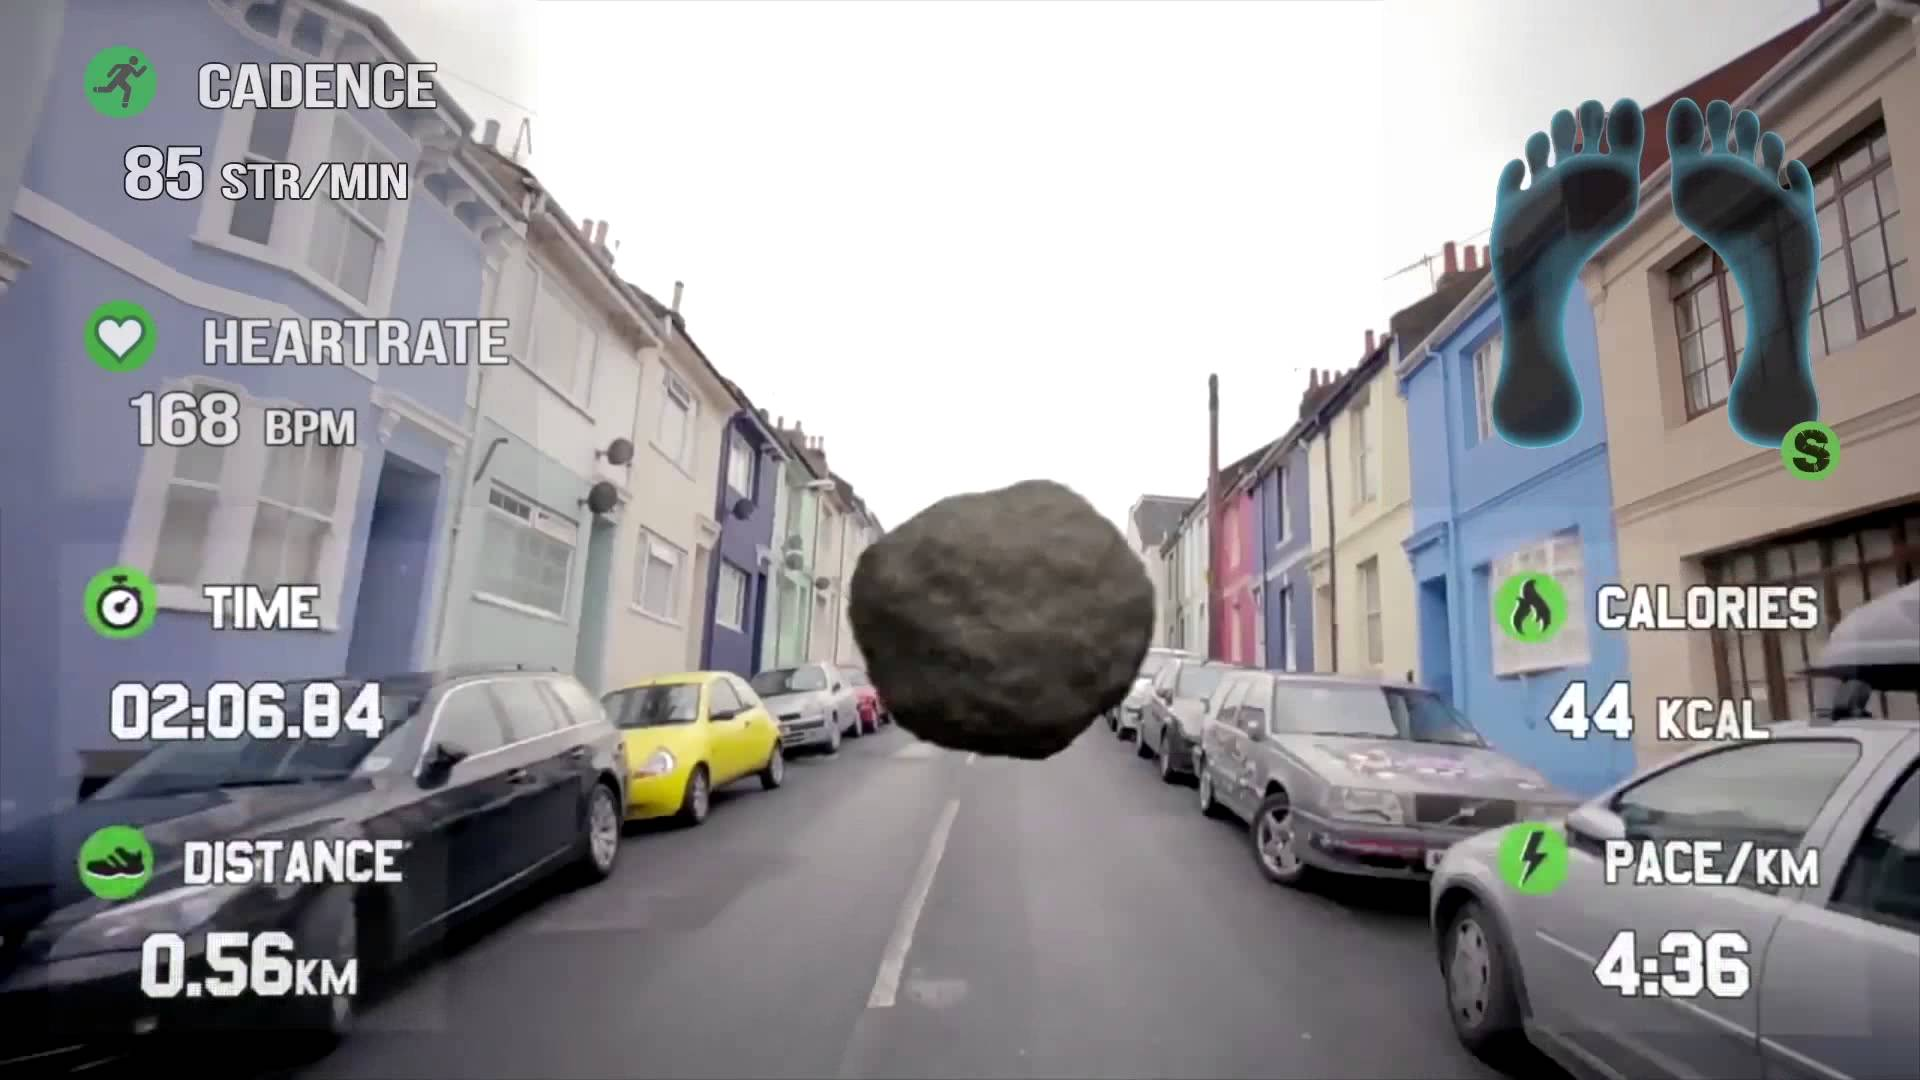
\includegraphics[width=0.6\linewidth]{googleglass}
	\caption{Google Glass. Demostración de su uso en deportes}
	\label{fig:googleglass}
\end{figure}

\subsubsection{Tipos de RA}

Existen hoy en dia cuatro tipos de RA.

\begin{itemize}
	\item 
	Marker-bases AR. Se basa en el reconocimiento de imágenes conocidas como marker o marcadores. Los marker son imágenes distintivas que son reconocidas por nuestro dispositivo facilmente ya que contienen puntos visuales únicos. Un buen ejemplo de este tipo de imágenes son los conocidos código QR\cite{URL::CodigoQR}, también tiene usos en el reconocimiento de textos para su traducción o para crear simulaciones de objetos 3D o arquitecturas sin llegar a construirlas de forma física. RR

	\begin{figure}[h]
		\centering
		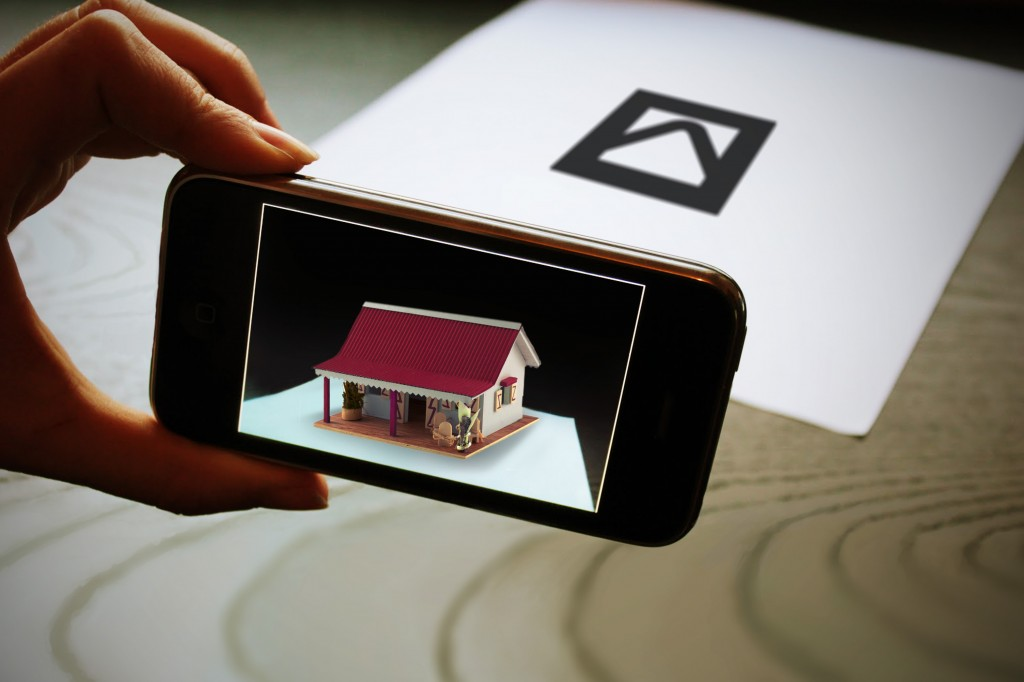
\includegraphics[width=0.6\linewidth]{marker-ar}
		\caption{Marker-bases AR. Demostración de su funcionamiento}
		\label{fig:markerAR}
	\end{figure}

	\item Markerless AR. Corresponde a la RA que recoge los datos de su posición, orientación y localización para mostrar la información correspondiente a ese área. Estos sistemas utilizan los datos obtenidos del GPS, brújula, giroscopio y acelerómetro para establecer la ubicación del usuario. Este tipo de RA puede proveer de ayuda viajeros que necesiten una mano para moverse por la ciudad, ya que mediante el reconocimiento de su ubicación y la orientación pueden mostrarles la ruta para llegar a su destino o mostrarle información de los puntos de interés que les rodean. 
 
	\item Pojection-based AR. Este tipo de RA consiste en la proyección de luz en superficies y objetos en el mundo real. Existen muchos usos interesantes de esta tecnología, como aplicaciones para el uso de teclados virtuales proyectados que reconozcan cuando una "tecla" es pulsada. Esta proyección también se puede hacer en medio del aire con ayuda de la tecnología de láseres de plasma.

	\item Superimposition-based AR. Esta tecnología remplaza la imagen original por una de AR, de forma complete o parcial. El reconocimiento de objetos juega un papel fundamental en este tipo de tecnología. Tiene gran utilidad el campo de la medicina, por ejemplo un doctor podría examinar a un paciente mientras ve la imagen de RA que se creado a partir de una visión de rayos X y la imagen real de paciente, así puede ver y entender mejor el daño en un hueso.
\end{itemize} 


\subsubsection{Diferencias entre Realidad Aumentada y Realidad Virtual}
En los último años la Realidad Virtual(RV) \cite{URL::VR} o Virtual Reality(VR) en inglés y la Realidad Aumentada han empezado a recibir mucha más atención. Llevando a desarrolladores llevar acabo integraciones de ambas tecnologías en numerosas industrias.

De acuerdo a un análisis de expertos, decía que la RV iba tener el liderato por 2018 como tecnología pionera, sin embargo la RA va tener mucha mas importancia y a largo plazo, llegando a forma parte de nuestro día a día.

Realidad Virtual es un entorno de escenas u objetos de apariencia real. Aleja la usuario del entorno real y da la sensación de estar inmerso en él. Dicho entorno es contemplado por el usuario a través de un dispositivo conocido como gafas o casco de realidad virtual. Este puede ir acompañado de otros dispositivos, como guantes o trajes especiales, que permiten una mayor interacción con el entorno así como la percepción de diferentes estímulos que intensifican la sensación de realidad.

La Realidad Aumentada no aísla al usuario de mundo exterior, sino que lleva al mundo real objetos no existentes al mundo real mediante la superposición de imágenes en tiempo real.	

\subsubsection{Realidad Mixta}

Existe otro tipo de tecnología que nace de la unión de Realidad Aumentada y la Realidad Virtual, la Realidad Mixta(RM) \cite{URL::RM}. Es un tipo de realidad similar a la Realidad Aumentada pero con una idea mas ambiciosa de mezclar lo real con lo virtual. La RM es mucho mas inmersiva que la realidad aumentada y requiere de mucho mas poder de procesamiento.

Un ejemplo del uso de esta tecnología puede ser el mejorar los métodos de aprendizaje de los estudiantes, mediante simulaciones de tareas construidas virtualmente en un entorno real.  


\subsubsection{Futuro y usos de la AR}
Actualmente la Realidad Aumentada la tenemos mas mano que en años. Dispositivos como los smartphones ya nos traen y nos enseñan las primeras muestras de esta tecnología, la cual esta en sus primeros años de desarrollo pero ya se puede ver el potencial y la enorme importancia que va a tener en un futuro.

Los usos actuales de esta tecnología se acercan a todo los sectores conocidos:

\begin{itemize}
	\item Realidad Aumentada en Educación. La llegada de la RA afectara a los procesos convencionales de aprendizaje. La RA tiene la capacidad de cambiar el horario y el lugar en el que se estudia y la posibilidad de introducir nuevos métodos de enseñanza. 
	
	Actualmente gran parte de la población joven tiene un smartphone el cuál es un medio hábil para la RA. Por lo tanto se dan unas condiciones idóneas para que la RA profundice en el campo de la Educación y se hagan más descubrimientos ya que cada estudiante va a tener un dispositivo a mano capaz de reproducir la RA,lo cual puede ayudar a los estudiantes a tener contenidos mas accesibles sobre cualquier asignatura o conseguir que información compleja sea más fácil de entender. Un ejemplo claro sería la creación de libros interactivos que la ser apuntados con las cámara del móvil muestren el funcionamiento en 3D de un volcán o del latido de un corazón.

	\begin{figure}[h]
		\centering
		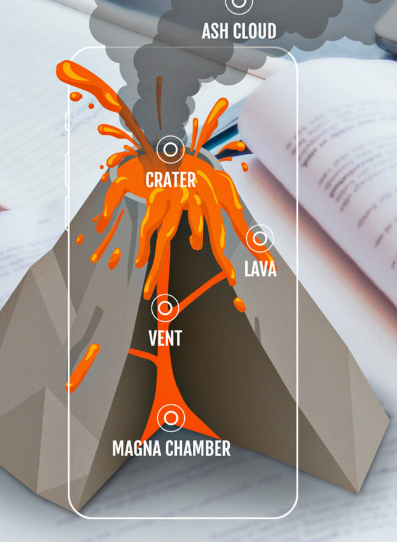
\includegraphics[width=0.6\linewidth]{education-example}
		\caption{RA Volcán. Ejemplo de uso de RA en Educación }
		\label{fig:education-example}
	\end{figure}

	\item Realidad Aumentada en Turismo. El negocio del turismo siempre ha intentado estar al dia con la nueva tecnología para poder ofrecer nuevos servicios, formas de publicitarse, transporte y actividades de ocio. Por eso no es raro que la RA se haya hecho un hueco en este sector debido al potencial que tiene para mejorar la experiencia de los turistas. 
	
	Posibles usos en este sector son la puesta de guías turísticas que faciliten a los usuarios de estas moverse por la ciudad, señalando puntos de interés, datos históricos, restaurantes, hoteles, etc. El mismo concepto podría aplicarse en museos y zoos. Otro uso interesante sería el de romper la barrera del lenguaje gracias a la traducción inmediata de señales, textos y anuncios, al idioma del turista. 

	\item Realidad Aumentada en Medicina. En cuanto a la Medicina, es interesante ver como avanza la tecnología en este campo pero a su vez es bastante difícil de prever que tipo de ventajas nos ofrecerá.
	
	Los principales usos que se plantean se encuentran enfocados principalmente en los quirófanos, en los que el especialista o cirujano monte una especie gafas-pantalla que le permita realizar la operación sin la necesidad de apartar la vista del paciente para consultar información o ir monitorizando la operación. Esto se traduce en operaciones mas rápidas y seguras sin que el cirujano se despiste. A su vez esto podría mostrar información anatómica sobre el paciente en tiempo real,  es decir gracias a algoritmos de inteligencia artificial permitir identificar nervios, venas mayores y huesos y que esto sean marcados con un distinto color, facilitando mucho las labores de los médicos.

	\item Realidad Aumentada en los Videojuegos. Uno

\end{itemize}


\subsubsection{AR SDK en Android Studio}

\begin{itemize}

	\item Vuforia Es un SDK disponible para todas la plataformas(android, IOS, windows)y para Android Studio. Es muy potente para el desarrollo de aplicaciones de realidad virtual, ya sea para el reconocimiento de imágenes, escanearlas, reconocimiento de múltiples objetos, reconocimiento y superficies planas. Ademas también permiten el reconocimiento de acciones realizadas por el usuario para la interaccion con los distintos elementos disponibles. El uso de esta SDK esta principalmente enfocado para trabajar junto Unity.

	\item Kudan es el principal rival de Vuforia, facil de usar y eficiente, usa SLAM para el reconociento de objetos e imagenes. Tiene una licencia gratis para desarrolladores, una de sus desventajas es que tiene problemas con su key pare empezar a desarrollar y que a veces tiene problemas con el editor de Unity.

	\item EasyAr en su version Free, tienes soporte para todas la plataformas y para Android Studio. Contiene reconocimento de imagenes planas, reconocimiento de imagenes multiples con deteccion de refleco y oclusion, reconocimiento limitado de imagenes en la nube. Su version mas potente se llama SLAM y solo es disponible para la versión de pago.

	\item Maxst ofrece reconociento de objetos de imagenes, SLAM, multiplataforma, facil de usar. Optimizado para moviles, incluso con bajos recursos Se puede utilizar con android studio, tienen un plan para desarrolladores free, con acceso a la mayoria de funcionalidades de su SDK.
	\item 
\end{itemize}

\subsection{Nodejs}
\subsection{Mongodb}
